This exercise has been completed in the attached \textit{PCA and classification.ipynb} Jupyter Notebook. The most relevant bits of source code can be seen here as well, though all comments are left out. The full source code is in the notebook, along with comments:
\begin{verbatim}
def kfold(train, labels, x):
    retTrain = numpy.zeros(train.shape)
    retLabs = numpy.zeros(labels.shape)    
    perm = numpy.random.permutation(train.shape[0])
    
    for oldInd, newInd in enumerate(perm):
        retTrain[newInd] = train[oldInd]
        retLabs[newInd] = labels[oldInd]
        
    retTrain = 
        retTrain.reshape(x,
                         int(np.floor(train.shape[0]/x)),
                         train.shape[1])
    retLabs = 
        retLabs.reshape(x,int(np.floor(labels.shape[0]/x)))
    return retTrain, retLabs

def crossVal(train, trainlab, x, k):
    foldedArrs, foldedLabs = kfold(train, trainlab, x)
    
    accs = np.zeros(int(np.ceil(k/2)))
    nums = np.arange(1,k+1,2)
    
    for i in range(1,k+1,2):
        tempAccs = np.zeros(x-1)
        
        for j in range(x-1):
            tempTrain = 
                np.zeros((foldedArrs.shape[0]-1,foldedArrs.shape[1],foldedArrs.shape[2]))
            tempTrainLab = 
                np.zeros((foldedLabs.shape[0]-1,foldedLabs.shape[1]))
            
            tempTest  = np.zeros((1,foldedArrs.shape[1],foldedArrs.shape[2]))
            tempTestLab  = np.zeros((1,foldedLabs.shape[1]))
            
            for l in range(x):
                if (l<j):
                    tempTrain[l] = foldedArrs[l]
                    tempTrainLab[l] = foldedLabs[l]
                elif (l>j):
                    tempTrain[l-1] = foldedArrs[l]
                    tempTrainLab[l-1] = foldedLabs[l]
                else:
                    tempTest = 
                        foldedArrs[l].reshape(1,foldedArrs.shape[1],foldedArrs.shape[2])
                    tempTestLab = foldedLabs[l].reshape(1,foldedLabs.shape[1])
            
            tempTrain = 
                tempTrain.reshape((tempTrain.shape[0]*tempTrain.shape[1]),
                                   tempTrain.shape[2])
            tempTest = 
                tempTest.reshape((tempTest.shape[0]*tempTest.shape[1]),
                                  tempTest.shape[2])
            tempTrainLab = 
                tempTrainLab.reshape((tempTrainLab.shape[0]*tempTrainLab.shape[1]))
            tempTestLab = 
                tempTestLab.reshape((tempTestLab.shape[0]*tempTestLab.shape[1]))
            tempAccs[j] = 
                knn(tempTrain,tempTest,tempTrainLab,tempTestLab, i)[1]
            
        index = np.argmax(accs)
        accs[int(np.ceil(i/2))-1] = np.mean(tempAccs)

    return nums[np.argmax(accs)], accs, index
\end{verbatim}
When running these functions, we get the following results:
\begin{itemize}
	\item $k$ value for highest accuracy on training set: $21$
	\item $k_{best}$ accuracy on training set : $\sim 0.7650$
	\item Accuracy of $k$-$NN$ against test set with $k=k_{best}$: $\sim 0.7531$
\end{itemize}
We see that the accuracy of $k$-$NN$ with $k_{best}$ is slightly more accurate than the originals we calculated in $5c$, but no much. We can also see that our $k$-$NN$ with $k_{best}$ performs slightly worse on the test set than on the training set. This is likely due to pure chance, as we would expect the model to perform the same, or slightly better since it has been trained on the entire training set, instead of only $9/10$ths of it.\\
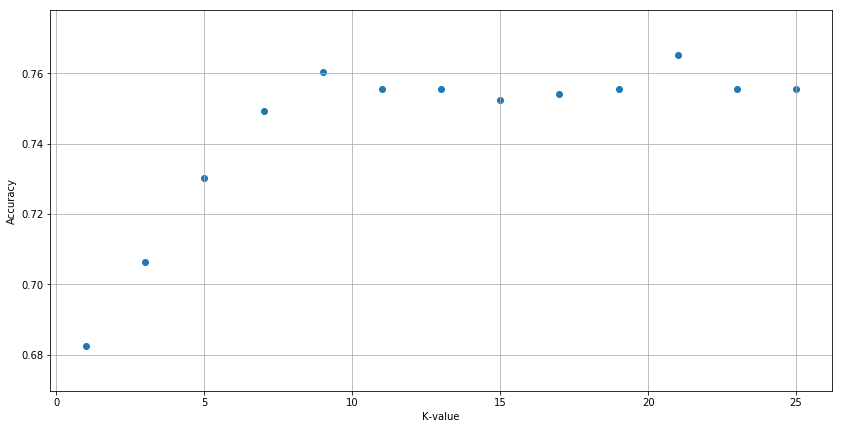
\includegraphics[width=\linewidth]{5d1.png}